\subsubsection{Support Vector Machines}
\textbf{S}upport \textbf{V}ector \textbf{M}achine eller SVM er en gren inden for supervised machine learning\cite{ML_BOOK}, som går ud på at inddele datapunkter i forskellige klasser. I forbindelse med selvkørende biler, kunne SVM blive brugt til at separere billister fra cyklister, og igen fra fodgængere.

SVM virker ved at indsætte datapunkter i et koordinatsystem, og så finde et `hyperplane' der kan skille de forskellige typer data fra hinanden. På figur \ref{fig:SVM} ses et koordinatsystem hvor der er indtegnet to forskellige typer data, som ønskes adskilt. For at adskille de to typer data på figur \ref{fig:SVM}, kan der bruges en lineær funktion. Det kan ses på illustrationen, at linjen $h_1$ ikke adskiller de to datasæt, og derfor ville dette hyperplane ikke virke. $h_2$ adskiller de to datasæt, men med en meget lille margin. Til sidst har vi så $h_3$ som adskiller de to datasæt med en stor margin, her vil der altså være størst sandsynlighed for at en computer kunne forudsige hvilken gruppe datapunktet hører til. 
\begin{figure}[h!]
	\centering
	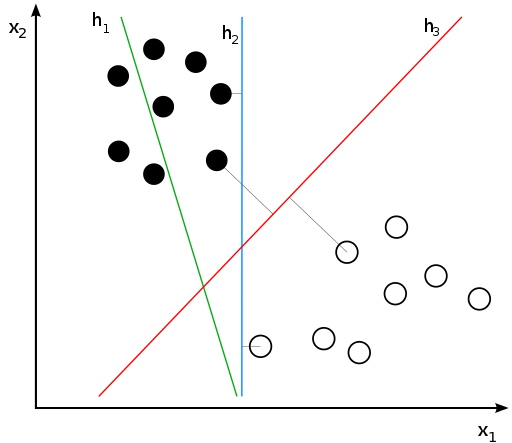
\includegraphics[width=0.6\textwidth]{images/SVM.png}
	\captionsource{Illustration af SVM}{\url{https://en.wikipedia.org/wiki/Support\_vector\_machine\#/media/File:Kernel\_Machine.png}}
	\label{fig:SVM}
\end{figure}

Kort sagt kan man altså sige at SVM går ud på at opstille et hyperplane med størst mulig afstand til de nærmeste datapunkter, da dette giver den største sandsynlighed for at computeren kan adskille dataet korrekt.
Når funktionen for hyperplanet er opstillet, vil den til en given vektor (som er datapunktet) give $h(\vec{x}) \geq 1$ hvis datapunktet ligger i den ene gruppe, hvorimod $h(\vec{x}) \leq -1$ hvis datapunktet ligger i den anden gruppe. 